\documentclass[a4paper]{article}

\usepackage[utf8]{inputenc}
\usepackage[polish]{babel}
\usepackage{polski}
\usepackage{listings}
\usepackage[margin=0.9in]{geometry}
\usepackage[usenames,dvipsnames]{xcolor}
\usepackage{lmodern}
\usepackage{pdfpages}
\usepackage{float}

\author{Dorian Janiak, Marcin Ochman}
\title{Sprawozdanie projektowe z Robotów Mobilnych nr 2}


\begin{document}

\maketitle

\newpage

\tableofcontents
\listoffigures

\newpage

\section{Wstęp}

Sprawozdanie projektowe obejmuje postęp prac od 15.04.2015 do 11.05.2015, które zostały wykonane przez wszystkich członków grupy tj. \textit{Doriana Janiaka} oraz \textit{Marcina Ochmana}. Podczas tego okresu zrealizowano następujące rzeczy:
\begin{itemize}
	\item została dopracowana aplikacja komputerowa wizualizująca ruch robota
	\item zakupiono i skompletowano elementy
	\item został uruchomiony moduł z mikrokontrolerem (NUCLEO STM)
	\item stworzono sterowanie silnikiem krokowym
	\item wykonano pomiar czujnikiem odległości 
	\item zlutowano sekcję zasilania płytki
	\item znaleziono dokumenty prezentujące sposób obsługi modułu Bluetooth HC05 oraz silnika krokowego 
\end{itemize}


\section{Opis wykonanych prac}

Poniżej zostały szczegółowo opisane prace, które wykonano na rzecz projektu.

\subsection{Prace projektowe nad aplikacją na PC}

Został zaktualizowany diagram klas oraz przypadków użycia występujących w aplikacji komputerowej. Zmienił się sposób organizacji klas oraz planowana funkcjonalność aplikacja została ograniczona (możliwość zapisu do pliku).

%\begin{figure}
%\centering
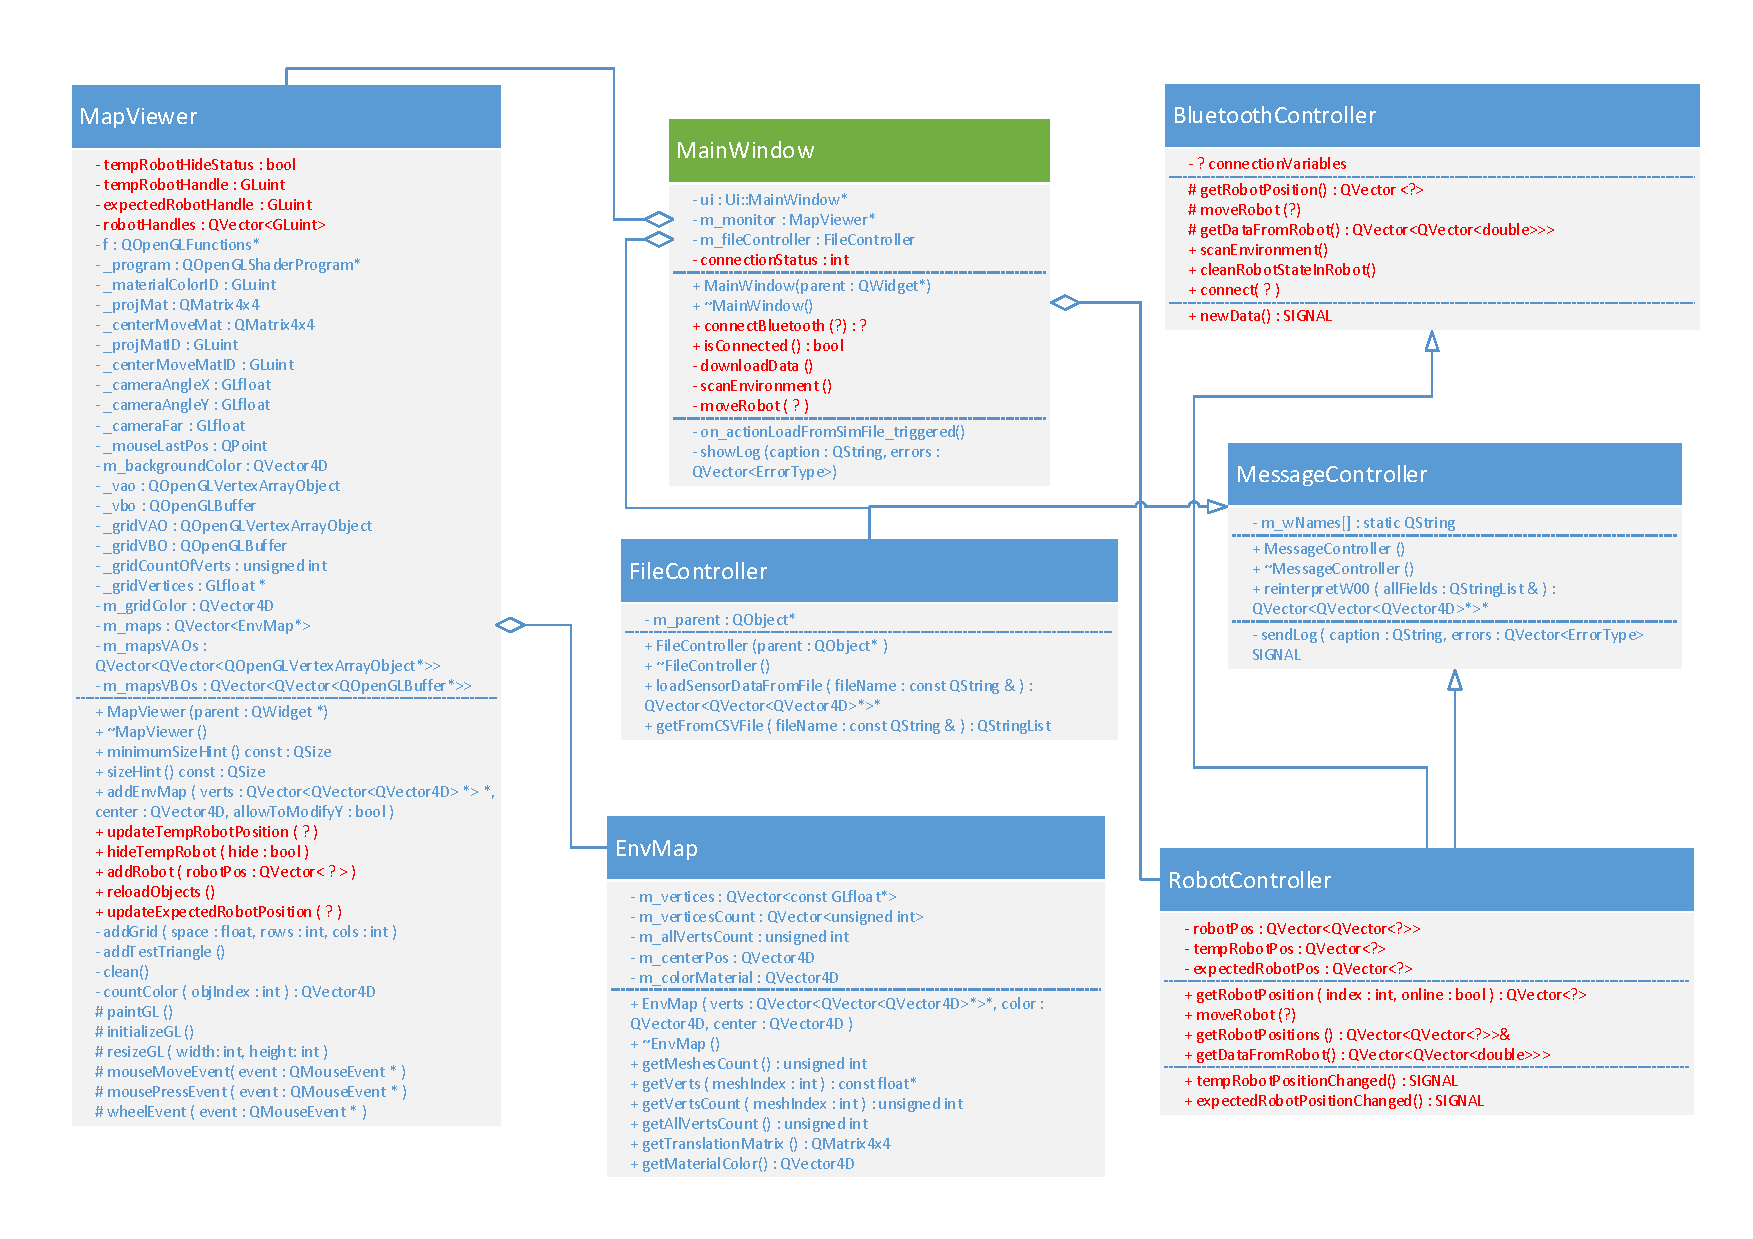
\includepdf[pages={1},landscape=true]{diagram_klas.pdf}
%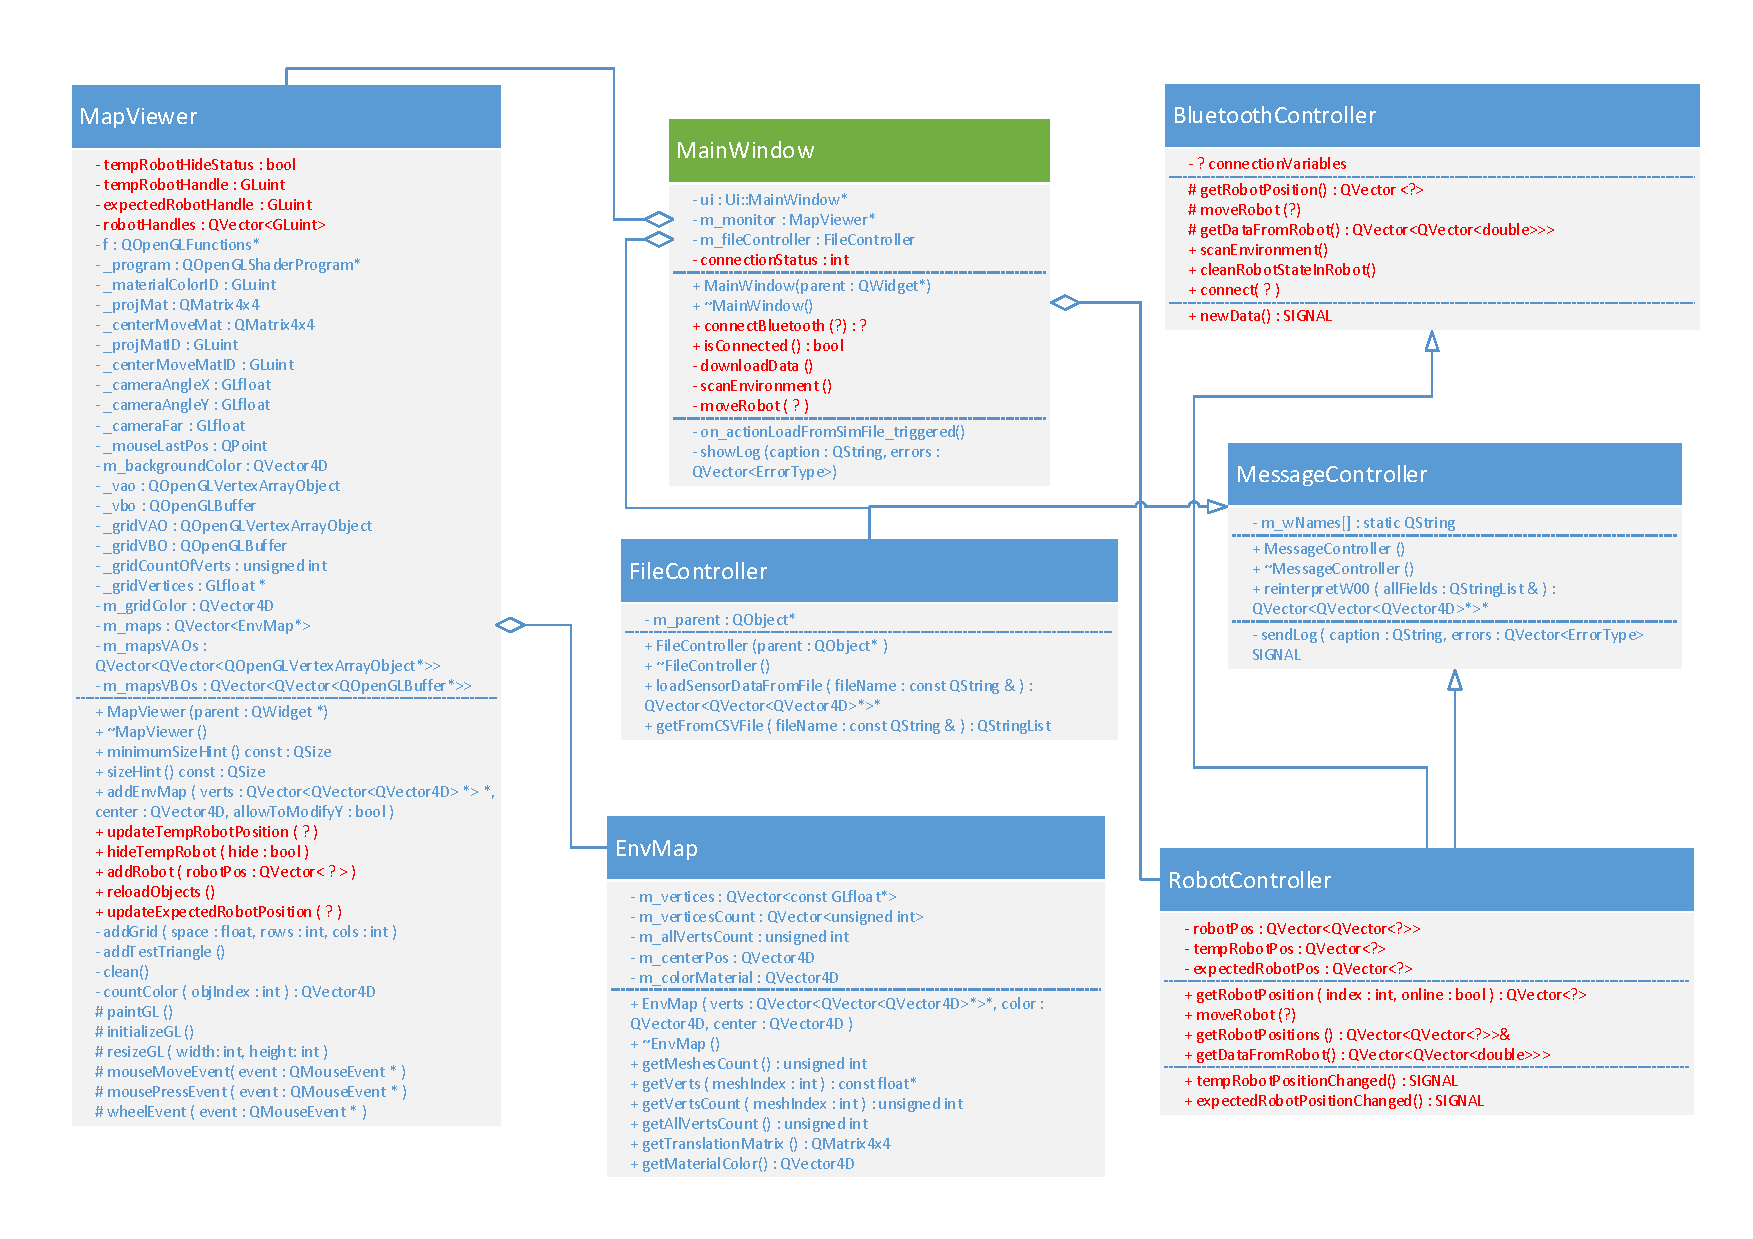
\includegraphics[height=0.9\paperheight, angle=90]{diagram_klas.pdf}
%\caption{Diagram klas aplikacji PC}
%\label{diagram_klas}
%\end{figure}

%\begin{figure}
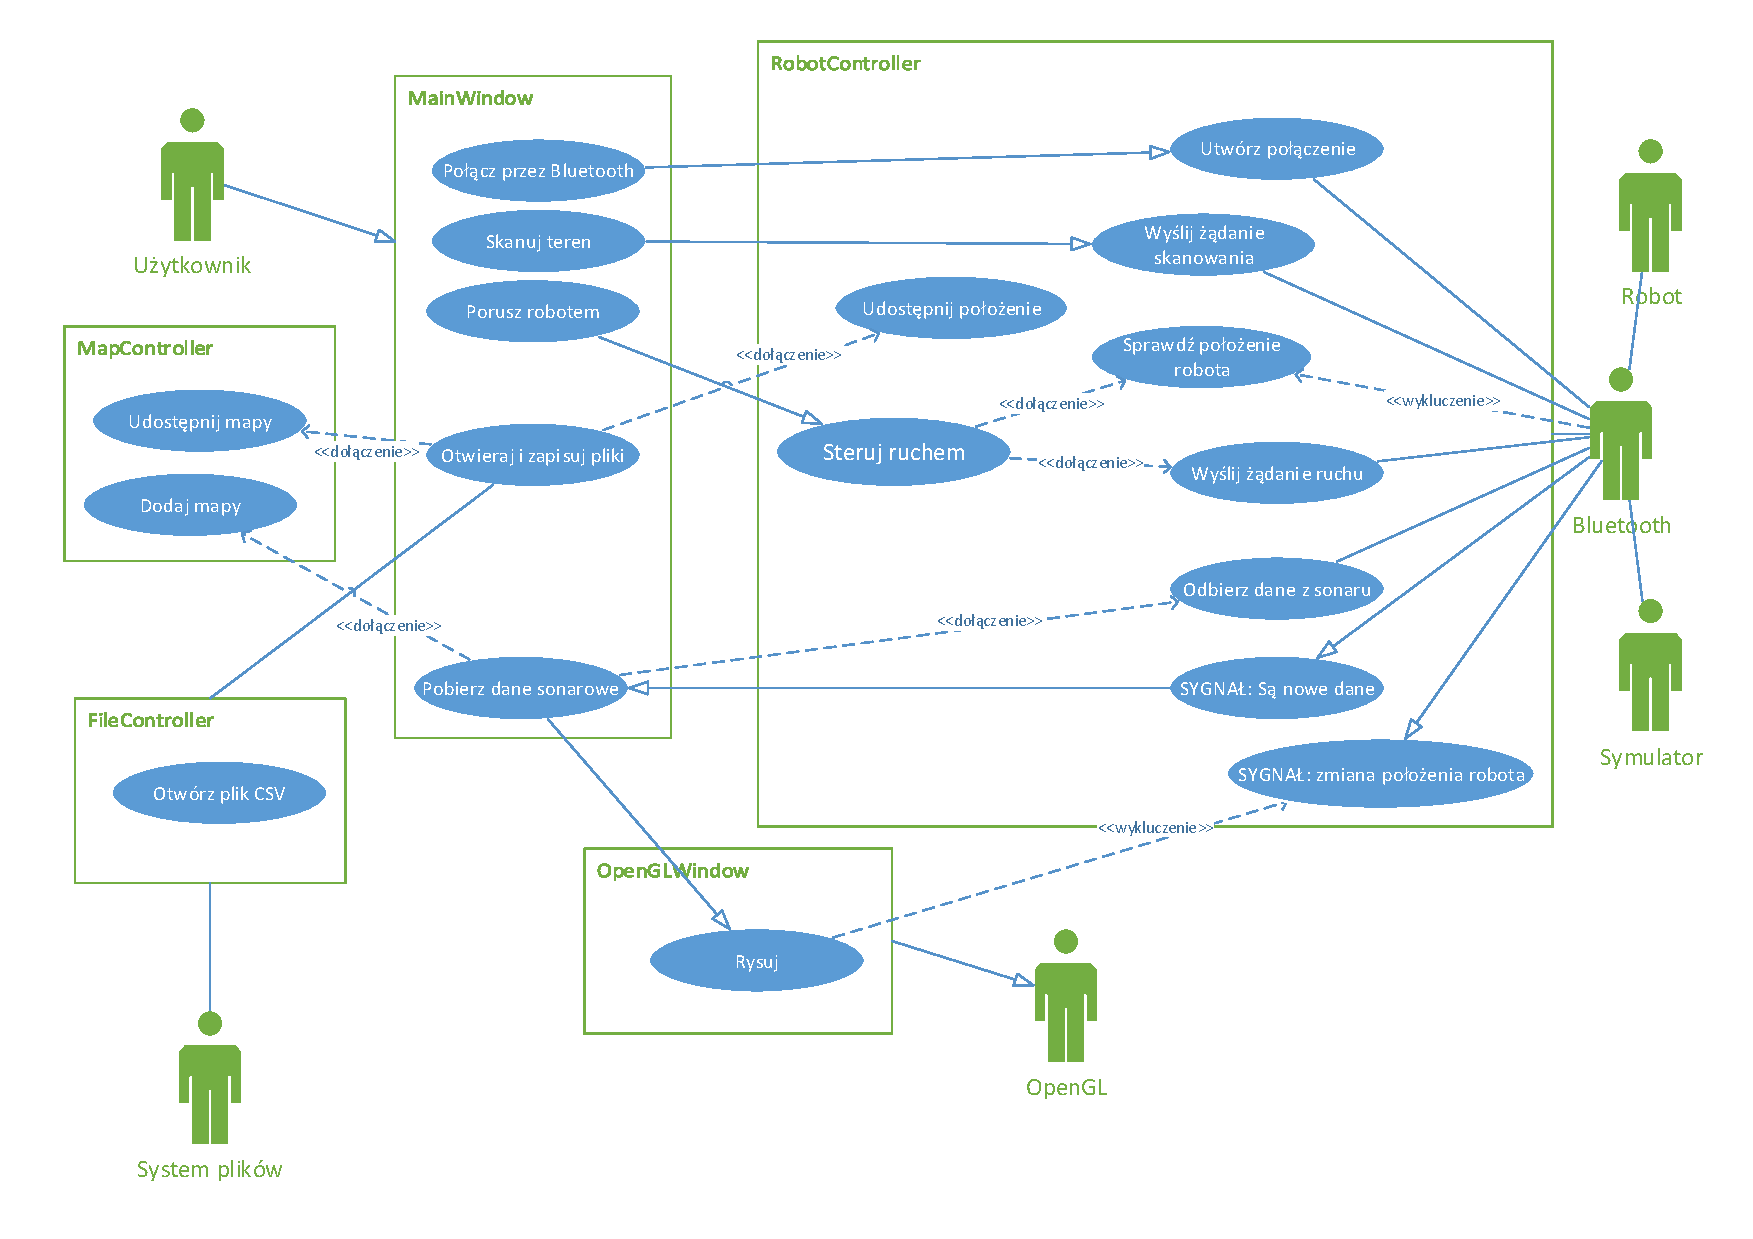
\includepdf[pages={1},landscape=true]{przypadki_uzycia.pdf}
%\centering
%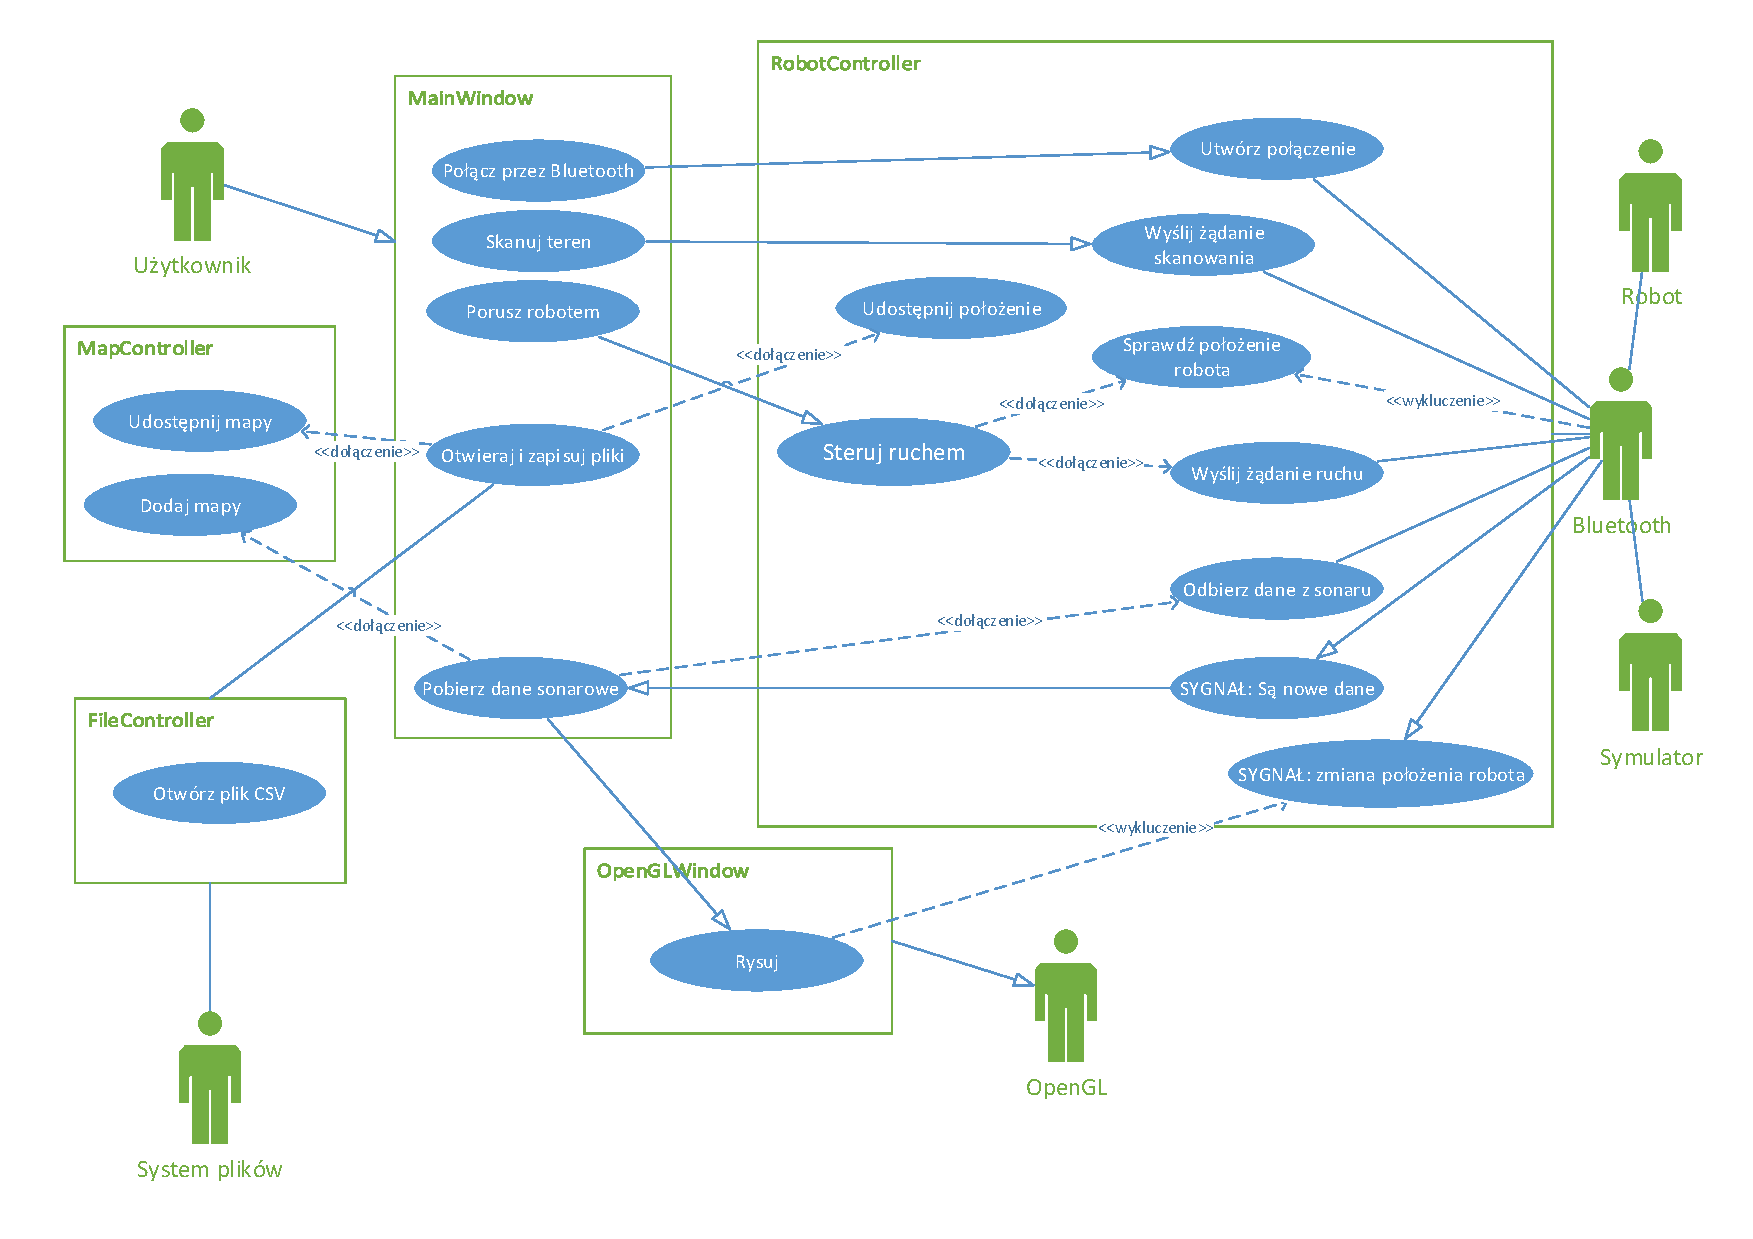
\includegraphics[height=0.55\paperheight, angle=90]{przypadki_uzycia.pdf}
%\caption{Diagram przypadków użycia dla aplikacji PC}
%\label{diagram_przypadkow_uzycia}
%\end{figure}


\subsection{Prace programistyczne nad aplikacją PC}

W określonym wcześniej okresie udało się przeogranizować strukturę aplikacji komputerowej, dzięki czemu jest ona znacznie bardziej uniwersalna. Dodana została możliwość sterowania obiektem, który ma służyć zadawaniu pozycji robota (dodano prosty graficznie pilot oraz możliwość załadowania obiektu 3D reprezentującego robota - na zruzcie ekranu żółty obiekt). \newline
Bardzo ważną funkcją aplikacji jest rysowanie mapy otoczenia. Na zrzucie obrazowana ona jest przez niebieską pogrubioną linię. Dotychczas aplikacja ładuje mapę z pliku.  
\newline
Dodatkowo utworzono widget, w którym znajdują się logi. W oknie tym pojawiać się będą pełne ramki otrzymywane poprzez Bluetooth, komunikaty błędów, ostrzeżenia, a także opcjonalne informacje związane przykładowo z obsługą robota. Okno to ma znacznie ułatwić późniejsze debugowanie komunikacji.  

\begin{figure}[H]
\centering
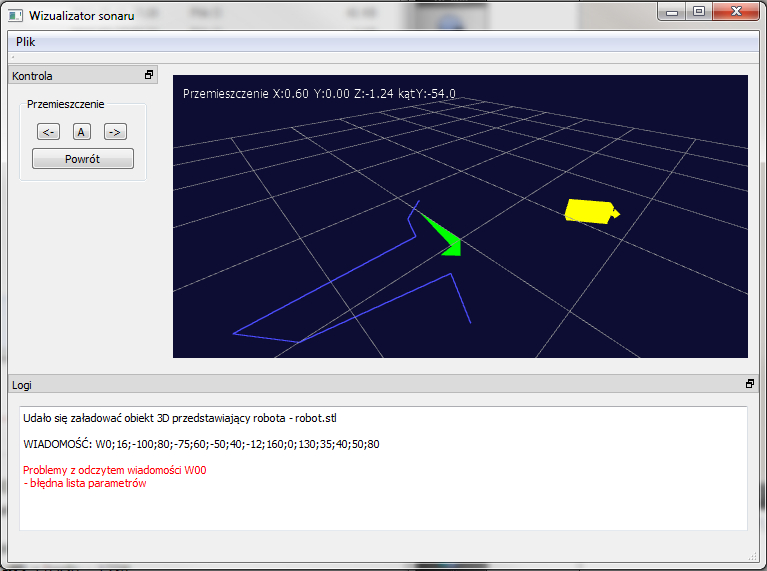
\includegraphics[width=\linewidth]{aplikacja}
\caption{Wygląd aplikacji}
\label{aplikacja}
\end{figure}

\subsection{Diagram dotyczący budowy robota oraz jego oprogramowania}

Na rysunku \ref{moduly_robota_pc} została przedstawiona komunikacja pomiędzy poszczególnymi modułami robota(zaznaczone na niebiesko). Diagram ten definiuje w jaki sposób będzie wyglądać sterowanie robotem oraz komunikacja pomiędzy komputerem osobistym. Widać, że za całe sterowanie będzie odpowiedzialny \textit{STM32}. To on będzie decydował jak mają poruszać się silniki, jak zostaną przetworzone informacje z enkoderów oraz czujnika ultradźwiękowego. Ostatecznie to on będzie odpowiedzialny za wysyłanie oraz odbieranie informacji i przetwarzanie komend przychodzących z komputera. Taka budowa definiuje w jaki sposób zostanie napisane oprogramowanie - każdy moduł sprzętowy będzie mieć własny moduł oprogramowania.
\begin{figure}[H]
\centering
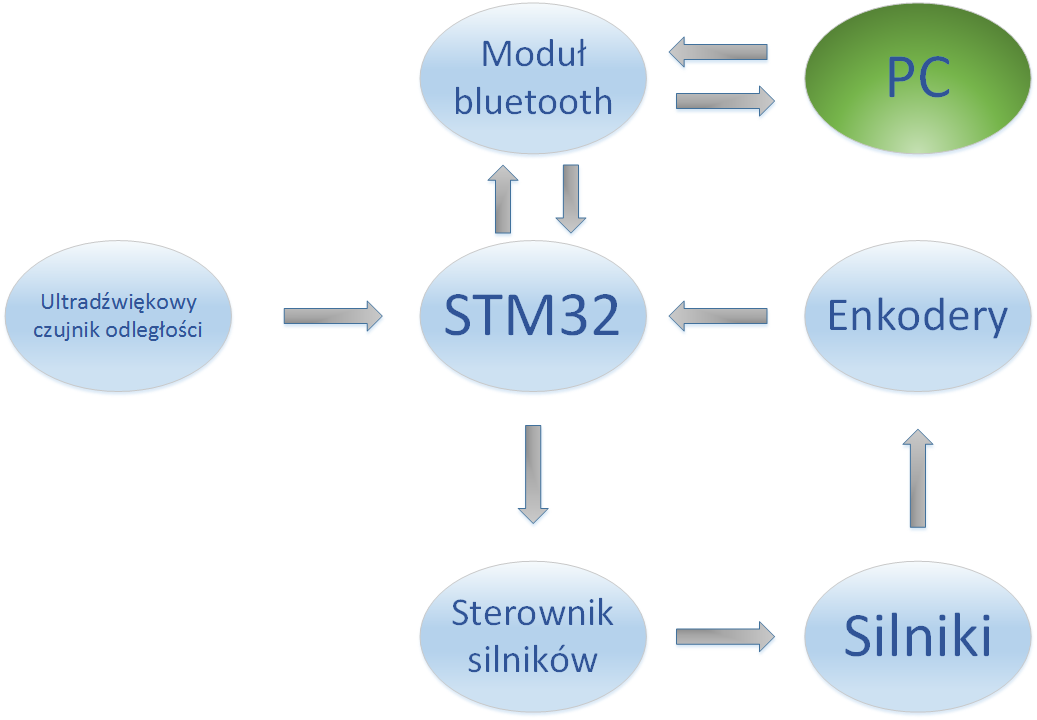
\includegraphics[width=\linewidth]{diagram_komunikacji_modulow_img}
\caption{Diagram przedstawiający moduły robota i PC oraz komunikację pomiędzy nimi}
\label{moduly_robota_pc}
\end{figure}


\subsection{Postęp prac przy budowie robota}

W opisywanym okresie udało się przede wszystkim zakupić większość potrzebnych do uruchomienia robota elementów. Do skompletowania pozostały elementy związane z samym stelażem robota. Poniżej wymienono postęp prac:
\begin{itemize}
	\item Uruchomienie płytki NUCLEO
	\item Stworzenie zasilania na bazie stabilizatorów napięcia 5V (model 7805) oraz 3.3V (model lm1117t) oraz płytki prototypowej.
	\item Sprawdzono działanie silników DC dostarczonych w zestawie Dagu RS034.
	\item Uruchomiono silnik krokowy i wysterowano przy użyciu sterownika ULN2003.
	\item Wykonano pomiar przy użyciu czujnika odległości (HC-SR04)
	\item Obsłużono zwykłą diodę LED oraz wysterowano diodę LED2 przy użyciu PWM.
\end{itemize}
Ponieważ stelaż nie został jeszcze zmontowany, wyżej wymienione prace odbywały się przy użyciu płytki stykowej. 

\subsection{Organizacja prac}
W ciągu najbliższego miesiąca będzie miała miejsce realizacja druga część zadania, polegająca na montażu robota. Wstępne testy zakupionych elementów pozwoliły nam ocenić zakres prac wymaganych do stworzenia robota. Poniżej w punktach zostały one przedstawione:
\begin{itemize}
\item Tworzenie programów dla mikrokontrolera STM32 zamieszczonego na płytce NUCLEO okazuje się stosunkowo proste ze względu na bogatość dostarczonej biblioteki. Ten etap prac nie powinien przysporzyć problemów.
\item Dokonanie pomiaru czujnikiem odległości HC-SR04 zostanie zrealizowane na bazie przerwań reagujących na zbocza rosnące i opadające.
\item Enkodery dostarczone w pakiecie Dagu RS034 pozwalają na odczyt binarny, a więc nie uda się odczytać kierunku ruchu kół. Również zostanie zrealizowane na bazie przerwań.
\item Obsługa modułu Bluetooth HC05 jest dobrze opisana w źródłach internetowych. Komunikacja z mikroprocesorem będzie odbywać się przy użyciu UART. 
\item Do sterowania silnikami zostanie wykorzystany mostek H. 
\item Sterowanie silnikiem krokowym odbywa się przy użyciu 4 pinów jednego z portów. Podawanie kolejnych wartości powoduje sterowanie silnikiem.
\end{itemize}
Kolejne zadania, które w związku z tym należy wykonać to:
\begin{itemize}
\item Zmontować stelaż robota.
\item Zbadać stosunek kąta wychylenia silnika krokowego w stosunku do sterowania w mikrokontrolerze.
\item Podłączyć mostek H i silniki oraz stworzyć algorytm jazdy.
\item Odczytać dane z enkoderów oraz stworzyć algorytm wyznaczania aktualnego położenia.
\item Rozpocząć komunikację poprzez Bluetooth.
\item Magazynować dane pomiarowe.
\item Utworzyć klasę BluetoothController w aplikacji komputerowej, która obsłuży komunikację Bluetooth.
\end{itemize}


\section{Podsumowanie}

W czasie pomiędzy pierwszym, a aktualnym raportem nie udało się wykonać wszystkich planowanych prac. Zebrana została większość potrzebnych elementów robota. Budowa podwozia nie została jeszcze rozpoczęta, ale zostało rozpoczęte zadanie nr 4 umieszczone w harmonogramie (Oprogramowanie robota - komunikacja oraz sterowanie). Jednak tworzenie programów dla modułu NUCLEO jest znacznie prostsze dzięki gotowej bibliotece obsługującej wejścia i wyjścia. Przy tworzeniu harmonogramu nie było to uwzględnione. \newline
Aplikacja komputerowa została prawie ukończona. Należy jedynie dodać moduł Bluetooth oraz kontener, który zapamięta poszczególne pozycje robota, w których wykonywane były pomiary. 

\section{Materiały źródłowe}

Naszym głównym źródłem informacji do stworzenia aplikacji były strony dokumentacji technicznej bibliotek - \textit{Qt5} oraz \textit{OpenGL}. Strony główne zostały zamieszczone poniżej:

\begin{itemize}
\item http://doc.qt.io/qt-5/reference-overview.html
\item https://www.opengl.org/documentation/
\end{itemize}

Natomiast do obsługi modułów robota zosały wykorzystane informacje zawarte pod poniższymi adresami:

\begin{itemize}
\item http://www.mlodedrwale.pl/2013/07/05/tani-modul-bluetooth-cz1/
\item http://www.python.rk.edu.pl/w/p/sterowanie-silnikami-krokowymi-i-serwomechanizmami-za-pomoca-pymcu/
\item http://www.bajdi.com/adding-encoders-to-those-cheap-yellow-motors/
\end{itemize}

\end{document}
